\documentclass{article}
\usepackage{minted}
\usepackage[utf8]{inputenc}
\usepackage{graphicx}
\usepackage{float}
\usepackage{blindtext}
\graphicspath{{deliverables/proposal/}}

\title{SYSC 4907 Project Proposal : Smart Rollator}
\date{}
\author {Corbin Garlough - 101101493 \\
Kenny Deng - 101122713 \\
Isabelle Bryenton - 101077788 \\
Mark Johnson - 101110080 \\
Yunas Magsi - 10111515Project Objective}

\begin{document}
\begin{titlepage}
   \begin{center}
       \vspace*{1cm}
       \large
       \textbf{Smart Rollator - Capstone Project Proposal} \\
       \vspace{0.5cm}
       \normalsize
        SYSC4907, Group 33
       \vspace{4cm} \\
       \textbf{By: \\
            Corbin Garlough - 101101493 \\
            Kenny Deng - 101122713 \\
            Isabelle Bryenton - 101077788 \\
            Mark Johnson - 101110080 \\
            Yunas Magsi - 10111515} \\
       \vspace{2cm}
       \textbf{Supervised by: Dr. Adrian Chan \\}
       \vspace{4cm}
       Department of Systems and Computer Engineering\\
       Carleton University\\
       Ottawa, Canada\\
       October 21st 2022
   \end{center}
\end{titlepage}

\tableofcontents
\listoffigures
\listoftables
\newpage
\maketitle
\section{Introduction}
The Smart Rollator is a mobility aid that collects data about how a patient uses and moves with a rollator through multiple on-board sensors. A medical professional is able to monitor and adjust patient rehabilitation on a more continuous basis using collected data streamed to a cloud service for remote access. The goal of this project is to add sensors to a rollator, such as the Nexus rollator shown in \autoref{fig:1} in order to add functionality without modifying the design of the traditional rollator.

\begin{figure}[!h]
    \centering
    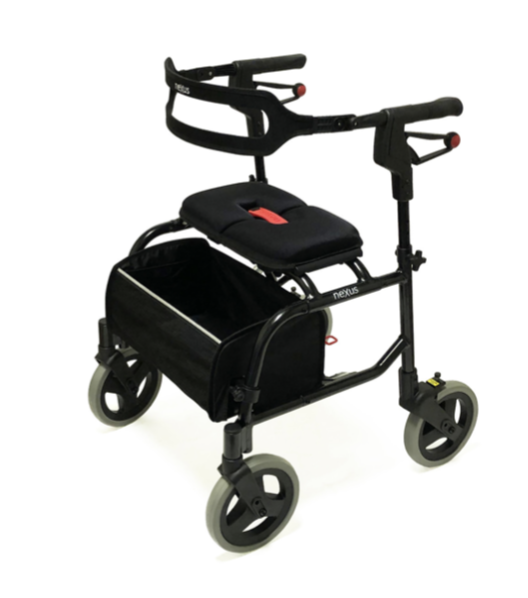
\includegraphics[scale=0.5]{nexus_rollator.png}
    \caption{Nexus rollator}
    \label{fig:1}
\end{figure}


\subsection{Justification of suitability}
Group 33 is a team composed of members with unique engineering backgrounds and skills which are well suited to the diverse requirements of the Smart Rollator project. Corbin, Kenny, and Yunas are Computer Systems Engineering students, Mark is a Software Engineering student, and Isabelle is a Biomedical and Electrical Engineering student. 

The computer systems degree is useful to this project because the degree focuses on the ability to integrate software and hardware together into a functional system. Since this project has multiple sensors, a cloud-based data storage system, and software to process data, the system integration skills learned in the computer systems degree will greatly assist in creating a final product. 

Similarly, Software engineering focuses heavily on the methodological aspects of writing software, including requirements engineering, system design documentation, verification and validation, and software quality management; all of these are important aspects of engineering and delivering correct and complete software  systems.  

Finally, a Biomedical and Electrical engineering degree will provide greater insight on the biomedical aspects of the project, given this is a medical device which utilizes multiple electrical sensors to acquire biomedical data, along with microprocessors to process and visualize the data.




\subsection{Team Member Tasking}
\autoref{fig:2} shows the distribution of the tasks for the project deliverables for each team member of group 33. 

\begin{figure}[!h]
    \centering
    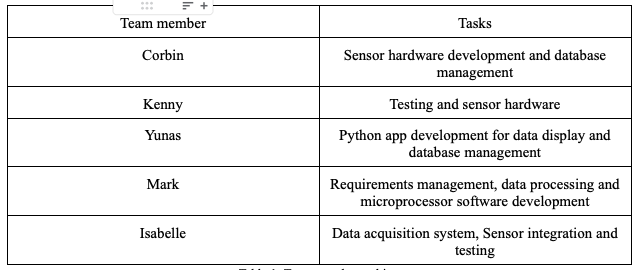
\includegraphics[width=0.8\columnwidth]{sysc4907_team_member_tasking.png}
    \caption{Team member Tasking for Project Deliverables}
    \label{fig:2}
\end{figure}

\subsection{Milestones}
\begin{itemize}
    \item Read data from sensors
    \item Mount sensors and required hardware to rollator frame
    \item  Export sensor data to cloud storage service
    \item Generate a summary of data viewing
    \item Have a patient use the rollator to collect data about a short period of activity
\end{itemize} \\
The milestones above have been documented in Jira, and assigned to the appropriate team member. \\ \\
\section{Methodology}
Group 33 is proposing the project be implemented to meet the following requirements, using the microprocessors, sensors and power supplies along with cloud data storage and analysis detailed in the following Implementation section of the proposal.

\subsection{Requirements}
\textbf{Functional Requirements} \\
The functional requirements are the features that provide the data of the rollator usage. These include motion sensing, usage time tracking, heart rate monitoring, weight sense applicator, power capacity to last a full day, and storage of local data, along with cloud upload.
Diving into motion sensing, the rollator must be able to track the speed at which the patient moves throughout the day, along with the distance traveled and average acceleration within it. The usage time is logged for the medical practitioner to see the frequency of use the patient is using the rollator, along with what position they are in, and whether they are seated, actively walking or stopped. The rollator will also include a Photoplethysmography-based (PPG) heart rate sensor, with which measurements will be taken from the patient throughout the day.
In terms of rehabilitation for the patient, there are 3 weight sensors of the rollator, one for each arm handle and one for the seating. These weight sensors are used to see if the patient has a preference for a side along with whether they are using the rollator while seated. With all these components within the rollator, power consumption is a factor that needs to be accounted for. The goal of the rollator is to include at least one full day's use, before needing a charge to have no extra burden on the patient. Ideally, all the data that is collected is stored within the rollator for approximately 5 days before it needs to be pushed to the cloud, this is for consideration of patients that have internet connection issues \\\\
\textbf{Non-Functional Requirements} \\
The power consumption patterns of the Smart Rollator are expected to be similar to those of consumer cell phones, with battery drain during the day when in use and battery charging required at night while idle, allowing more inexpensive charging solutions to be considered without impacting daily use. The rollator will require wired charging to minimize the technical barrier to entry for using the rollator, and to maximize the ease of use of the system. The Smart Rollator sensor modules and wiring will also be designed to allow the rollator to remain visually indistinguishable from a standard rollator while still remaining modular for future development, with a design intended to be as unobtrusive as possible for the patient; this is done to preserve the patient's dignity and not to bring unnecessary attention to them, as that may negatively impact the rehabilitation process by disincentivizing use of the rollator in public. The data analysis report will be designed for medical practitioners and will require patient-specific authentication to access. The report will be complete with regard to the collected data and will be simple to understand, allowing further work to be done on this aspect of the project in the future. \\ \\

\section{Implementation}
The requirements outlined above will be met by implementing the following hardware and software components as shown in the system diagram in \autoref{fig:3}.

\begin{figure}[!h]
    \centering
    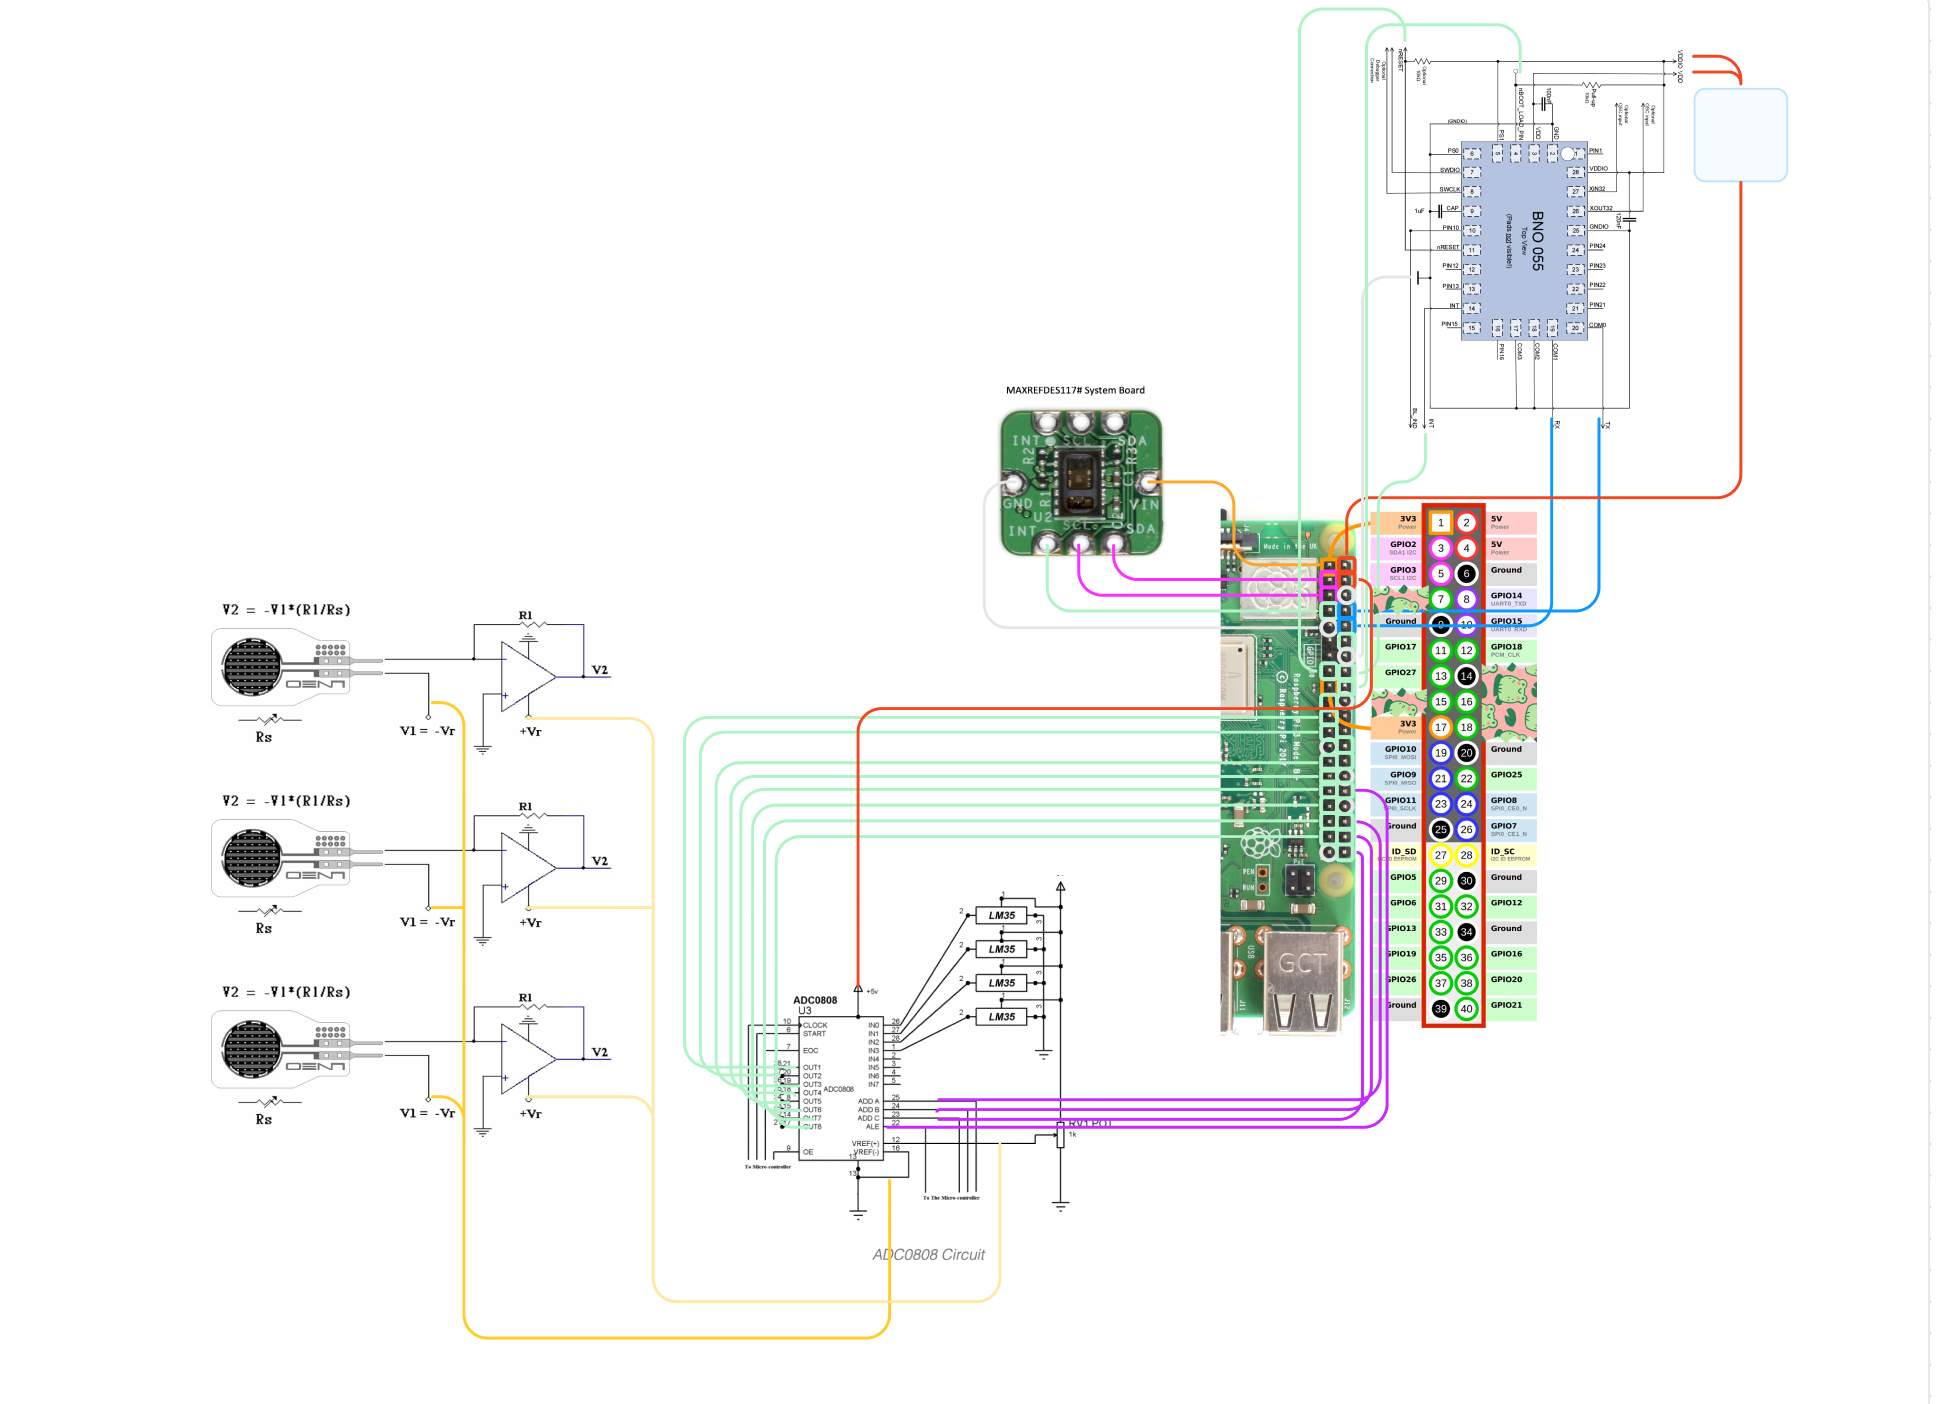
\includegraphics[scale=0.45 ]{sysc4907_system_diagram.png}
    \caption{RollSmart System Diagram}
    \label{fig:3}
\end{figure}


\subsection{Sensors}
\subsubsection{Heart Rate Sensor}
To measure the heart-rate of users while they are using the rollator a wired sensor PPG sensor has been chosen to be mounted on the handles of the rollator.
The MAXREFDES117 sensor that is a PPG optical heart-rate sensor (red and IR LEDs) which communicates using I2C. This sensor was chosen because of its low power consumption, small form factor (able to be mounted and placed on hand/finger), open-source heart rate and blood oxygen saturation level algorithm, and easy to connect terminals. PPG sensors are very reliable and accurate in determining heart rate. With a non-intrusive sensor there is minimal interference to the user (user places a hand over the sensor, not mounted to the user like a chest-mounted monitor and the user does not have to exert any additional effort to use the sensor). The flexibility is provided to us by the sensor in terms of mounting to the rollator (able to mount wherever the user has skin contact with the rollator). The sensor is readily available to ship at online vendor DigiKey.

When your heart beats, capillaries contract and expand. These contractions and expansions alter the volume of blood in the capillaries. The PPG heart-rate sensor emits red and IR LED light to detect and calculate these changes in blood volume and translates these changes into a heart rate. One heart rate sensor will be mounted on each of the rollator’s handles and constantly monitor the user’s heart rate through measurements of the user’s fingers/hands. The heart-rate sensor will be physically wired to the microprocessor.

\begin{figure}[!h]
    \centering
    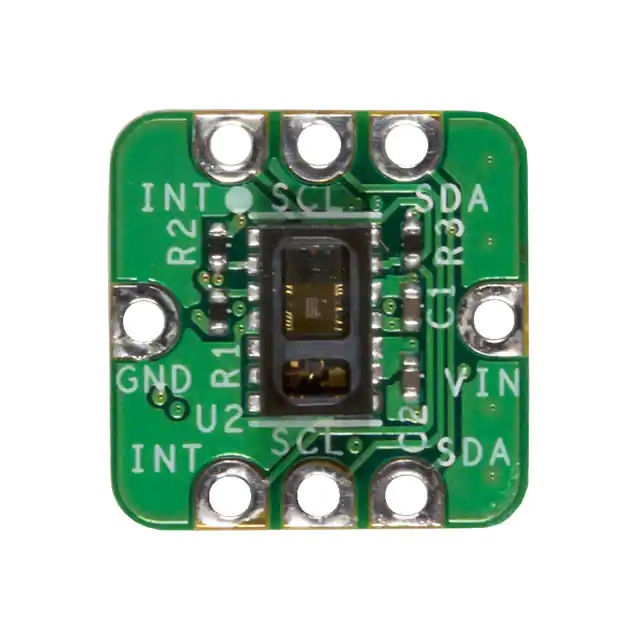
\includegraphics[scale=0.25]{sysc4907_MFG_MAXREFDES117.jpg}
    \caption{MAXREFDES117: Heart-Rate and Pulse-Oximetry Monitor}
    \label{fig:4}
\end{figure}

\subsubsection{Momentum Sensor}
The momentum sensor chosen is an IMU sensor, it will be used primarily to detect movement to track usage time, orientation and relative movement. The Bosch BNO055 IMU sensor shown in \autoref{fig:5} consists of multiple integrated sensors: an Accelerometer, Gyroscope and Magnetometer to function as a 9 axis sensor using I²C or SPI Output. This sensor was chosen for its form factor (small, chassis mounted), low power requirement, and dedicated mounting holes. The sensor is readily available to ship from the online vendor DigiKey. An alternative BNO055 sensor is available that Professor Chan had previously proposed due to having pre-existing hardware on hand.

\begin{figure}[!h]
    \centering
    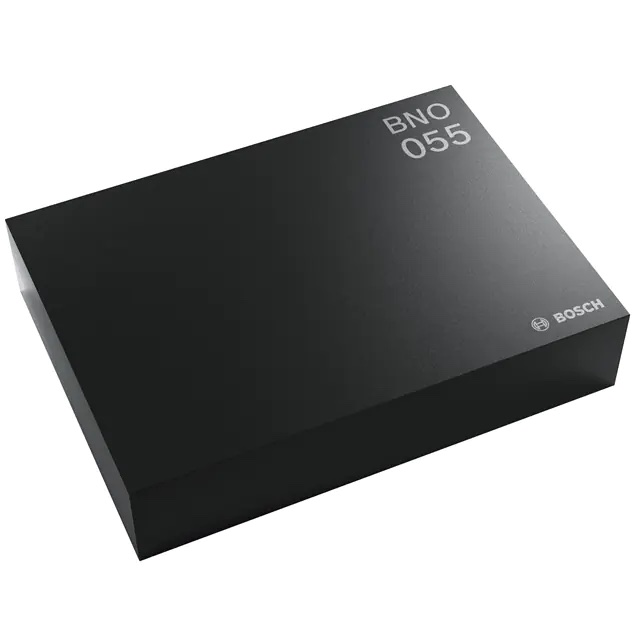
\includegraphics[scale=0.25]{MFG_BNO055.jpg}
    \caption{BMX160 9-AXIS SENSOR MODULE}
    \label{fig:5}
\end{figure}


\subsubsection{Speed Sensor}
A speed sensor will be used aboard the rollator to determine distance and speed travelled by the user during their rollator activity.
The existing rollator provided to us already has a speed sensor attached to the wheel/chassis. Since a sensor already exists we could reuse the old sensor and/or purchase a new one. We chose the MS-322-5 sensor because it is simple, small, compact, readily available on DigiKey and has 2 pre-existing mounting holes (easier to place in tight/small wheel well).

The magnet that is attached to the wheel(s) of the rollator and sensor detects revolutions of the wheel(s). The magnetic field produced by the magnet induces a current in the sensor wires and the sensor detects 
the induced current. With a predetermined measured circumference of the wheel, a speed can be derived. An option is to use two-speed sensors to detect the direction of travel. This can work in conjunction with the Momentum Sensor (9-axis IMU) for more accurate monitoring of distance and rollator use.

\begin{figure}[!h]
    \centering
    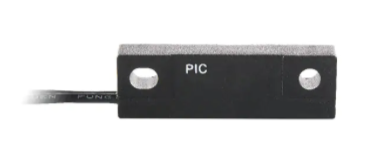
\includegraphics{MS_3225.png}
    \caption{MS-332-5: Mains Switching Reed Sensor Flatpack}
    \label{fig:6}
\end{figure}

\subsubsection{Pressure Sensor}
As pressure is applied to the surface the resistance of the metal decreases, which allows the determination of the force applied to the sensor. Three force sensors will be placed on the rollator in order to gain important information on the user's weight distribution when using the device. The first two force sensors will be placed under each of the handle grips of the rollator, in order to monitor the weight distribution across the rollator. Interesting data such as the user’s Left/Right balance can be determined by comparing the force recorded at the left and right handle sensors. 

The final force sensor will be bigger, and placed under the seat of the rollator. The data from this sensor will be used to determine the amount of time the user spends sitting down during a rollator ‘activity’. 

In brief, the force sensor will be used to determine if the smart rollator user has an equal Left/Right distribution when using the device, and how much time is spent sitting when operating the device. This data can be compared over time for interesting clinical applications, such as monitoring the progression of a patient over time to determine the efficiency of current treatment/rehabilitation protocols. 
\begin{figure}[!h]
    \centering
    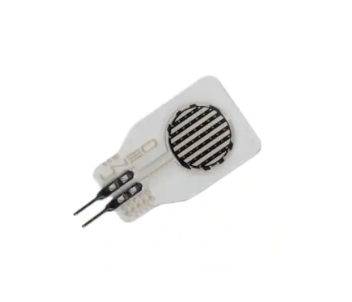
\includegraphics[scale = 0.7]{GHF_10.png}
    \caption{UNEO Inc, GHF-10 1cm Diameter Ultra Thin Flex Sensor
}
    \label{fig:7}
\end{figure}

\subsection{Microprocessor}
The microprocessor chosen for the Smart Rollator is the Raspberry Pi 4. After extensive research on various micro-controllers and microprocessors. It became clear that the Raspberry Pi offers a substantial amount of GPIO pins, computational power, Wifi/Bluetooth connectivity, can be used for threading operations more simply, and many more features. The Pi offers the best performance and flexibility. Should there be wireless sensors used, the Pi is more than capable of handling the new task. The Pi has a built-in real-time clock , which a lot of other microprocessors do not offer built-in. The Raspberry Pi runs its own operating system which is Linux based, meaning we can use the device as a regular computer if desired. 


\subsection{Powering The Rollator}
The rollator requires an independent power source to supply power to the microprocessor and the various connected sensors. What kind of battery and recharging system should it entail? We must consider form factor, ease of use, repairability, and upgradability.

The easiest most off the shelf solution is to use an existing Lithium Polymer portable battery bank product available on the market with a micro USB cable directly powering the Raspberry Pi 4 microprocessor. One cable from the microprocessor<->power bank for supplying power. One cable from the power bank <-> user for charging. This solution is very intuitive and can be easily modified in the future based on the increasing/decreasing power needs of the user. Very readily available and easy to replace (batteries have limited usable lifespan, having a self contained power unit makes it easy to replace).


An example of an existing readily available generic Lithium Polymer battery bank along with 36.6 Ah power capacity and input/output specs is shown in \autoref{fig:8}
(36.6 Ah, $36.76. Solar powered. 4 USB-A output (5V, 2.1A). 1 USB-C input/output (5V, 3A)) 
Purchase Link: https://www.amazon.ca/36800mAh-Outputs-Portable-Flashlight-Compatible/dp/B09YNL2V84/

\begin{figure}[!h]
    \centering
    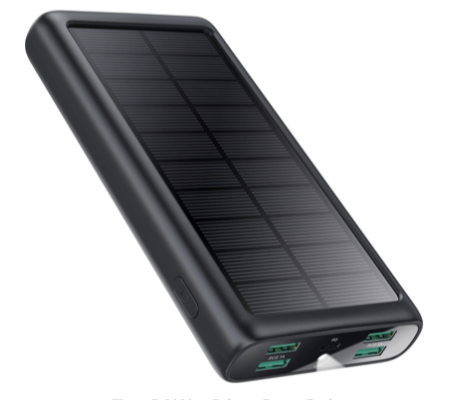
\includegraphics[scale=0.7]{lipo_battery.png}
    \caption{Lithium Polymer battery Pack}
    \label{fig:8}
\end{figure}


INSERT TABLE #3

From the proposed microprocessor and sensor hardware selection with an ~36 Ah Lithium Polymer battery pack we can expect ~12 hours of use between charges.

\subsection{Data Acquisition}
Data from the Smart Rollator sensor modules will be transmitted in several formats to the microprocessor for preprocessing, aggregation, and local storage in anticipation of being uploaded to a cloud-based storage backend for data analysis.
\subsubsection{Installation of sensors on Smart Rollator}
All of the sensors detailed above will be mounted to the Smart Rollator and hard wired into the GPIO of the Raspberry Pi. 

The Inertial Measurement Unit (IMU) supports both Inter-Integrated-Circuit (I2C) and Serial-Peripheral Interface (SPI) communication, of which we plan to use I2C due to its development simplicity and ease of integration with our chosen microprocessor. To ensure accurate data readings, the IMU will be mounted near the center of gravity of the rollator. 
The handle and seat strain gauges will transmit force readings as voltage differences between analog wire pairs, each connected to the GPIO pins of the microprocessor via Analog-to-Digital Converters (ADCs) in series with manufacturer-recommended LM358/LM324 operational amplifiers to translate the voltage input into a machine-readable format and reduce error from  the source impedance of the strain gauge as a voltage divider. 
The Reed switches will be mounted on the underside of the rollator wheel forks and connected to the microcontroller through analog wire pairs and ADCs, with readings transmitted as 500Hz current modulations induced by magnets embedded in the wheels for each fork. The Heart Oximetry Monitor (PPG) transmits data over I2C as well, and will be connected to the I2C bus of the microcontroller shared with the IMU.

\subsubsection{Collecting data from sensors}
The goal of the data acquisition device is to collect all the data gathered by the sensors, and package it into the desired format for processing and local storage. Once the data is stored, it will be pushed to the Cloud Database to be stored and analyzed.

Once the raw data inputs have been received in the microcontroller hardware buffers, they will be read by the Smart Rollator software and translated into a useful format for storage and transmission. Frequency measurements from the Reed switches will be averaged to reduce noise before being inputted into a wheel diameter-dependent equation to determine the speed of the rollator over its usage periods. However, the exact format of the strain gauge, PPG, and IMU readings have not yet been analyzed to determine what data preprocessing will be required prior to storage. Once an input data packet has been processed, it will be stored on a persistent flash storage medium connected to the microcontroller.

\subsection{Cloud Data Storage Back-end}
The Smart Rollator will use cloud-based storage to hold data collected about the patient, and allow a medical professional to view the data from anywhere. The cloud storage solution will be hosted on Google Firebase. The Raspberry Pi located on the rollator will upload collected data once a day when the device is put on charge. When the doctor wants to view the data, they will launch a python application that will pull new data from the cloud database. The system will require a username and password login for anyone attempting to view patient data. The database will have tables dedicated to storing information for an individual rollator, individual sensors, and all entries will have an associated time stamp.

\subsection{Data Analysis Application}
Once the rollator detects an activity is done, the data acquired during the rollator activity is pushed to the cloud backend. This is when the data analysis begins. When a medical practitioner would like to view the patient's data, they will have access to a desktop application. The desktop application shall have a login screen where the practitioner enters a username and password. The username and password are then compared to the cloud database where the username and password are authenticated. Once the session has been validated. The practitioner will be asked to choose which patient’s information they would like to view. Upon selection, the dataset will be presented. The practitioner will be able to choose from visualized data of the patient's movement throughout the day, the average pressure the user applies on the handle, and their heart rate throughout the day. These data points can be cross-checked with other data points for the medical practitioner to see if there is any correlation in the patient's day-to-day recovery.

\subsection{Testing}
\subsubsection{Unit Testing}
RollSmart, Test Smart. To achieve all the functional and non-functional requirements set out earlier in this proposal, it is imperative that each component of the project is continuously tested during every stage. Unit Tests will be implemented for each python script, and integrated into Github CI in order to continuously test the project’s code base. 

\subsubsection{Sample data for data analysis testing}
In order to test the Data Processing portion of the project, test data will be generated for each of the sensors on board the rollator, and used as input to the data processing sequence. The generated output will be tested to ensure it meets the requirements. 

\subsubsection{Continuous Integration, Delivery and Deployment (CI/CD)}
The project code base is hosted on Github, allowing all of the members to work on the project simultaneously with version control. Github also supports continuous integration and delivery (CI/CD), allowing automation of building, testing and integration of code changes in the repository and it's deployment. 
To improve CI efforts, a GitHub Pipeline has been implemented to pylint all files before they can be merged to main. This means that all code must comply with PEP8 standards before they can be incorporated into the main code base, ensuring that all the code which will be submitted for this project is robust and of high quality.

\subsubsection{RollSmart Test Fixture and integration into Github CI}
There will be a test RollSmart unit which will reside in the Lab, which will be equipped with all the RollSmart sensors and will be constantly connected to power and ethernet. It will  act as a remote test unit, where we can test hardware and software requirements. Ideally the RollSmart test unit will be integrated into GitHub CI as a worker, which will run the test sequence at desired intervals and when a merge request is triggered. This will allow the code to be continuously verified on the physical hardware with a simulated input, verifying any changes to new code which is getting committed to the code base. 

\section{Risk Analysis}
\subsection{Functional Safety}
The Smart Rollator is not a safety-critical system, and it makes no claims of compliance or attempts at conformance to development standards regulating such systems, including IEC:61508, IEC:62304, and IEC:60601. The existing design of the rollator will not be modified by the addition of sensors, we can assume the rollator functional safety will not be impacted by the sensors. Conducting a Hazard and Operability Analysis (HAZOP), a Failure Mode and Effect Analysis (FMEA), or an equivalent risk analysis methodology on the Smart Rollator design is therefore not in scope at this time. 

Given that such an analysis will not be performed, a Hazard and Risk Analysis (HARA) to document the hazards, risks, mitigations, and residual risks identified from such a risk methodology will not be developed, and no Safety Manual (SM) will be written to document the terms under which the Smart Rollator system can be used in accordance with its residual risks. 

\subsection{Quality Management}
The Smart Rollator project is vulnerable to a variety of common problems that may impact the delivery of the system, including implementation and testing difficulties from poor requirements, misunderstood allocations of tasks, bugs in the software or the hardware, and interpersonal conflicts between team members. These risks are mitigated in the Smart Rollator project through the use of industry-standard project management techniques and tools to manage the scope, schedule and cost of the project, and the responsible application of engineering expertise to distribute project responsibilities and decide on the project design.

Project requirements are organized hierarchically through Atlassian’s JIRA software, with stakeholder requirements created to document the intentions of the project, system requirements created for our design strategy to satisfy the stakeholder requirements, and software and hardware requirements created for the implementation details of each system requirement, all of which have bidirectional traceability between one another. Individual tasks are assigned to members of the project, and are linked with specific requirements, allowing progress on the project to be tracked both from a high-level and low-level perspective, and clearly indicating gaps in either the requirements or the development efforts project members are engaged in. The project schedule is also integrated with the requirements and task tracking system to clearly indicate which tasks must be completed by what dates, and to keep the team on track.

\section {Budget}
A bill of materials is outlined in \autoref{fig:9}, listing all the components required to implement the smart rollator design. \\

\begin{figure}[!h]
    \centering
    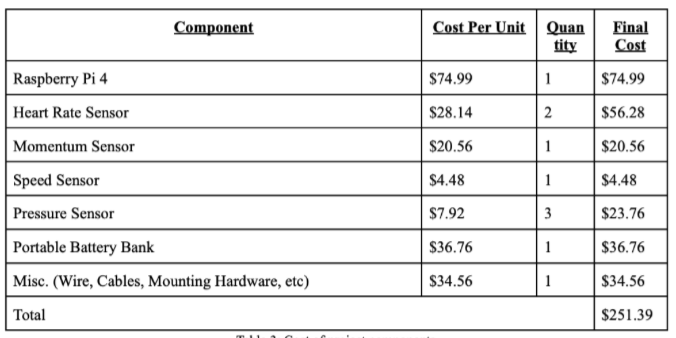
\includegraphics[scale=0.92]{sysc4907_BOM.png}
    \caption{Bill of Materials for Smart Rollator}
    \label{fig:9}
\end{figure}



\section{Project Timeline}
The Smart Rollator has a lot of rolling parts that need to come together. From the stakeholder requirements to the sensors, data acquisitions, hardware, cloud, and data reports. There are 4 main categories for the project including planning, building, development, and testing. The Gantt Chart in \autoref{fig:10} displays the general timeline which we aim to follow to accomplish the project.
\begin{figure}[!h]
    \centering
    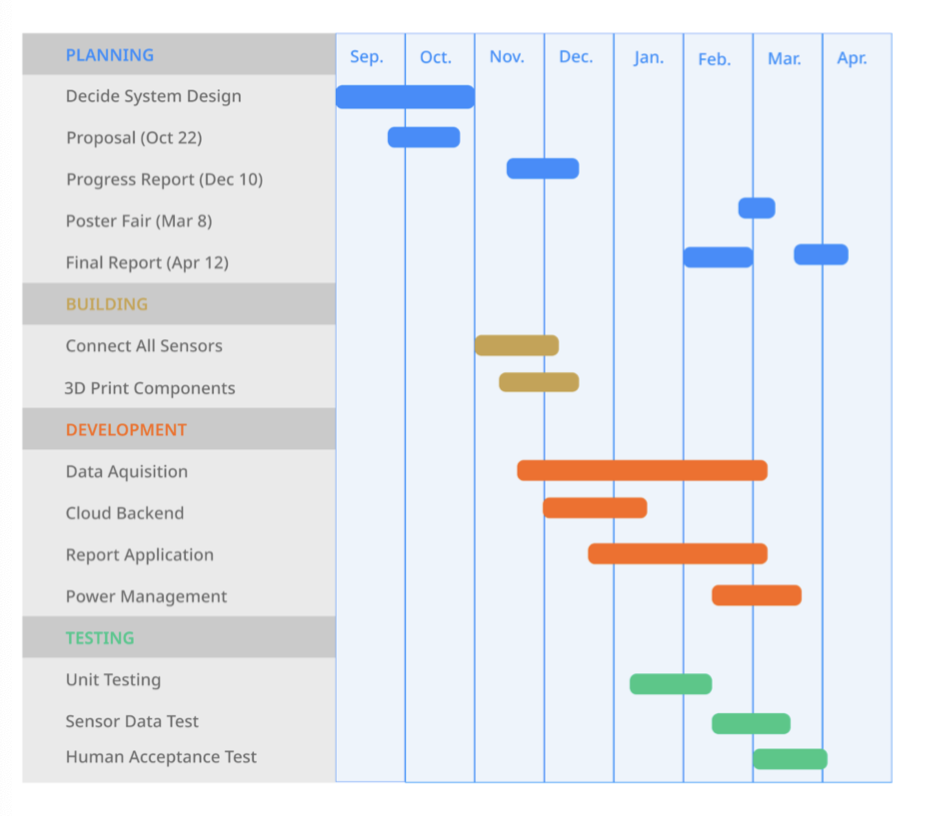
\includegraphics[width=0.8 \columnwidth]{sysc4907_gantt.png}
    \caption{Smart Rollator Project Timeline}
    \label{fig:10}
\end{figure}

These milestones have been assigned to a Team member who willl act as the Milestone Lead. The lead for each milestone will be responsible to the organization of the work and for distributing tasks to other team members. Another important role of the milestone lead wil be to ensure that all the requirements which were outlined in tis proposal are being met. \autoref{fig:11} shows a breakdown of the Milestones and their respective team lead. 

\begin{figure}[!h]
    \centering
    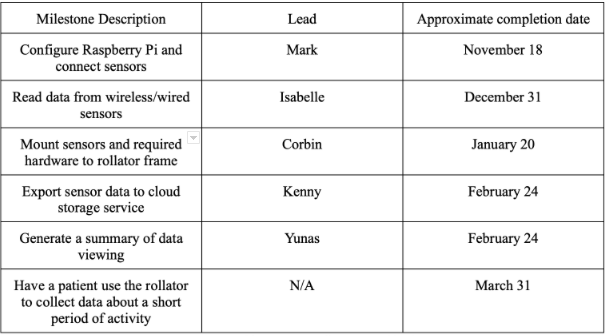
\includegraphics[scale=0.7]{sysc4907_milestone_leads.png}
    \caption{Breakdown of Milestones and team leads}
    \label{fig:11}
\end{figure}

\newpage
\section{Conclusion}
The Smart Rollator is a project which requires the exploration of various engineering principles, such as 3D printing, biomedical sensors and their implementations in microprocessor applications, cloud data storage, data processing and CI/CD. The aim of this project is to add sensors to a rollator which provide an abundance of useful clinical data for Doctors to determine treatment efficiency and monitor patient health over time. These additional electronic components will be hidden as best as possible on the rollator in order to minimize the disruptions to the user and have been chosen to minimize the cost and energy requirements. The data provided by the smart rollator will allow doctors to have a better understanding of their patients daily movements and exercise patterns and how their biometrics are affected by rollator usage. With its modular design, it can be retrofitted between different styles of rollators, which will in turn upcycle the rollator to sustain the environment. This project will offer the creators of the Smart Rollator an adventurous experience and training in engineering projects. With that, group 33 is proud to present the Smart Rollator.

\end{document}
